\section{Context}
\label{sec: Context}
\begin{figure}[h]
    \centering
    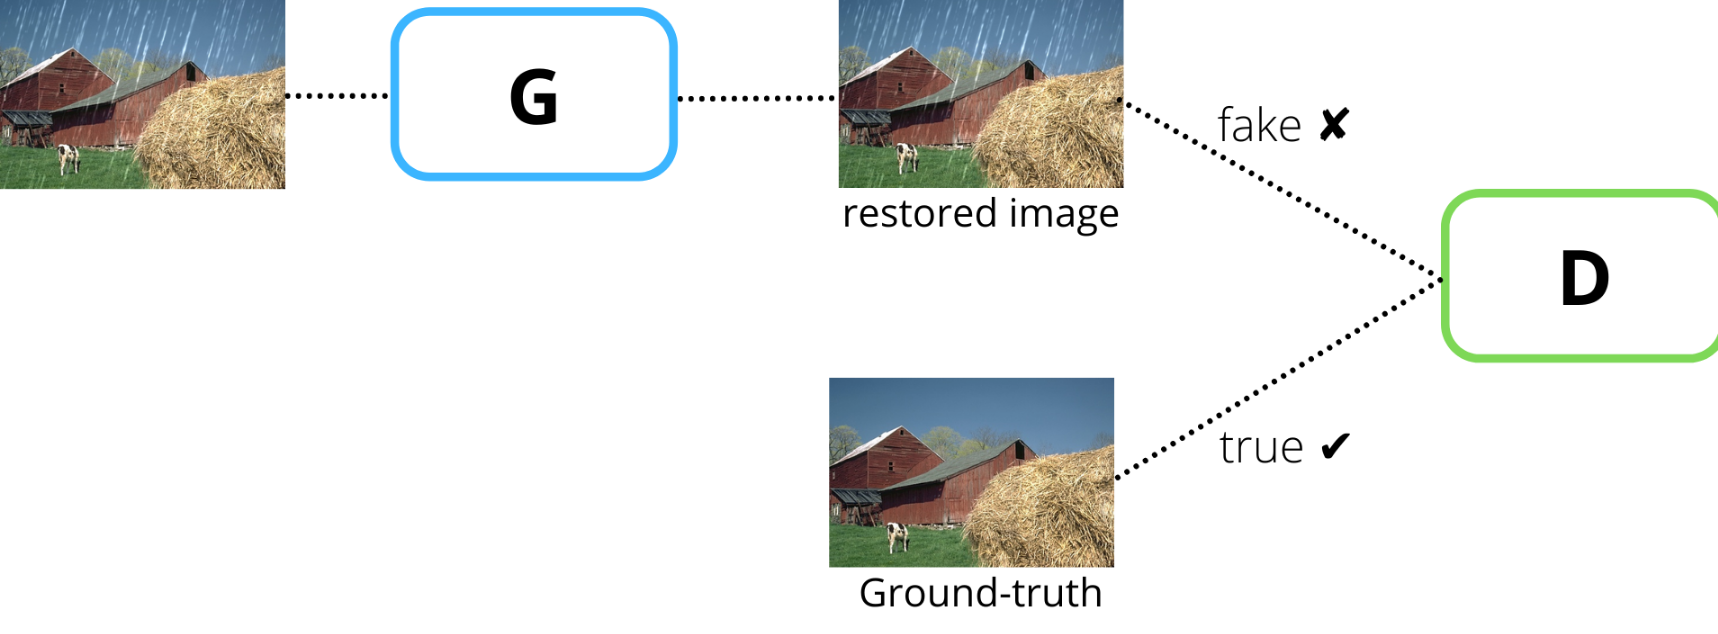
\includegraphics[scale=0.23]{./figures/sup_GAN.png}
    \caption{Supervised approach for image restoration through a GAN framework.}
    \label{fig: sup_GAN}
\end{figure}
In the context of self supervised images restoration I have recently explored Generative Adversarial Network (GAN) to train image restoration models in an unsupervised fashion. This aligns with the philosophy of image-to-image translation which learns the mapping of from an input image to an output images \cite{isola2017image}. In this context the goal is to learn the mapping from degraded images $Y$ to clean outputs $X$.
\par In a supervised fashion, the task would be for the generator $D$ to take as input degraded images $Y$ and generate $D(Y)$ a restored (fake) image. Then, a discriminator $D$ take on the role learn the restored (fake) images from the clean ground-truth $X$ as shown in Figure~\ref{fig: sup_GAN}.
\begin{figure}[t!]
    \centering
    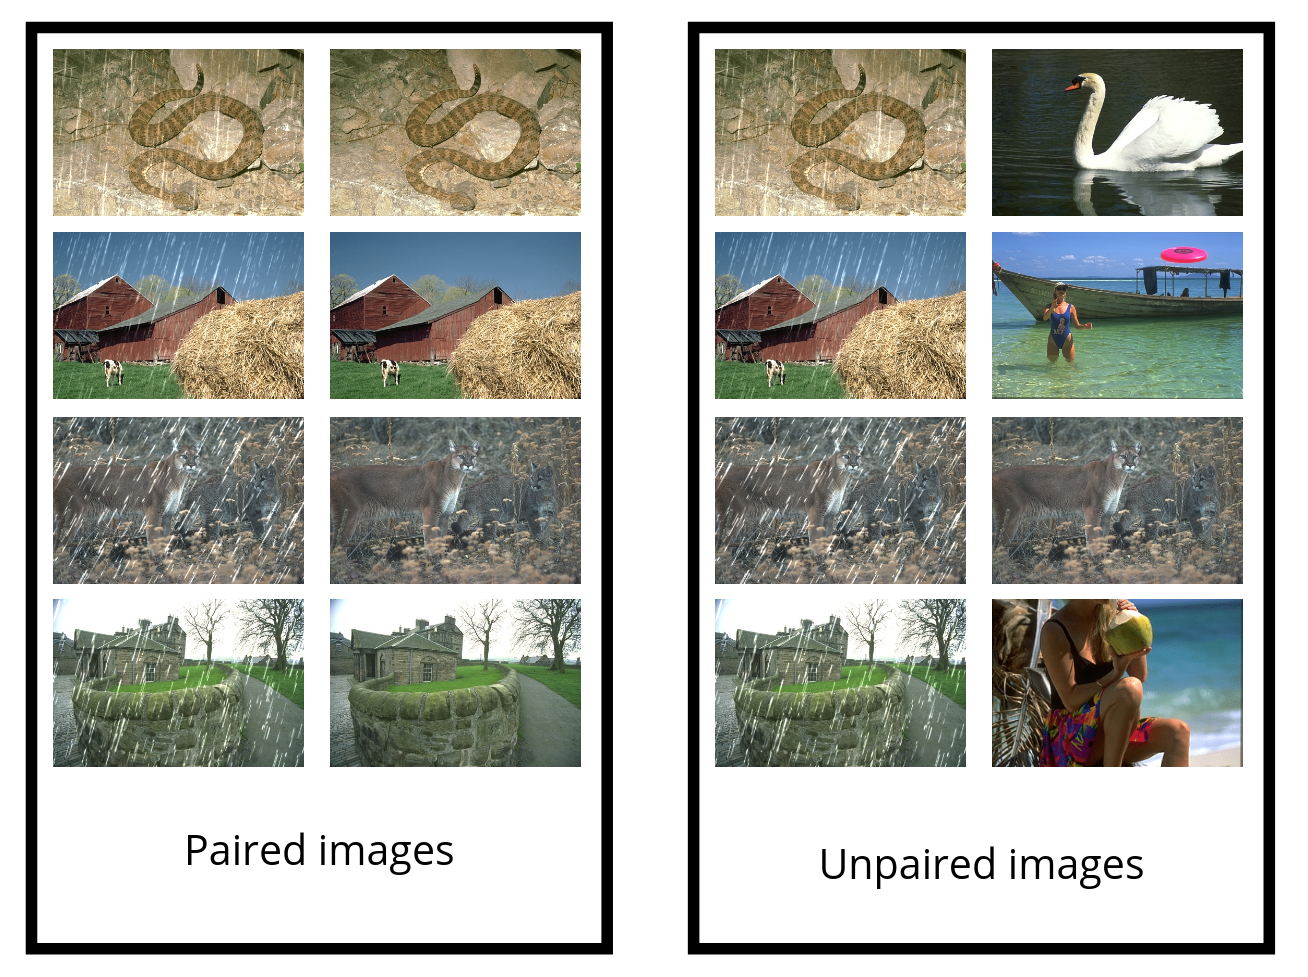
\includegraphics[scale=0.2]{./figures/pairs.png}
    \caption{Paired and paired images for training.}
    \label{fig: pairs}
\end{figure}
\par It is also still possible to achieve image restoration without having access the paired corrupted-clean images. The GAN generative models showed impressive performance when it comes learn the distribution of a given set of images. We can train our model learn to differentiate between corrupted and clean images without necessarily having access to paired data Figure~\ref{fig: pairs}. Thus, the discriminator would learn to differentiate corrupted natural images from clean ones. And hopefully signaling the generator to generate restored images and achieving self supervised image restorations.
\par Therefore, we can reformulate the GAN restoration problem as training a generator to restore clean images by only looking at unpaired corrupted-clean images as depicted in Figure~\ref{fig: unsup_GAN}.
\subsection*{ViT and Robustness}
\par Vision Transformers (ViT) have gain a lot of attention in the computer vision community since the seminal work of Dosovitskiy \etal \cite{dosovitskiy2020image}. Further works \cite{bai2021transformers} have extensively explored the robustness of ViT on out-of-distribution benchmarks \cite{hendrycks2018benchmarking}. As quoted on their paper
"\emph{The dominion of CNNs on visual recognition has been challenged by the recent findings that Transformers appear to be much more robust than CNNs. For example, Shao et al. \cite{shao2021adversarial} observe that the usage of convolutions may introduce a negative effect on model's adversarial robustness, while migrating to Transformer-like architectures (e.g., the Conv-Transformer hybrid model or the pure Transformer) can help secure models’ adversarial robustness. Similarly, Bhojanapalli et al. \cite{bhojanapalli2021understanding} report that, if pre-trained on sufficiently large datasets, Transformers exhibit considerably stronger robustness than CNNs on a spectrum of out-of-distribution tests (e.g., common image corruptions \cite{hendrycks2018benchmarking}, texture-shape cue conflicting stimuli \cite{geirhos2018imagenet}).}".
\subsection*{Assumption}
\par \emph{ViT might be a key feature for a self supervised GAN image restoration model. The built-in robustness of ViT to various degradation motivate us to explore its effectiveness combined with a GAN framework.}
\begin{figure}[h]
    \centering
    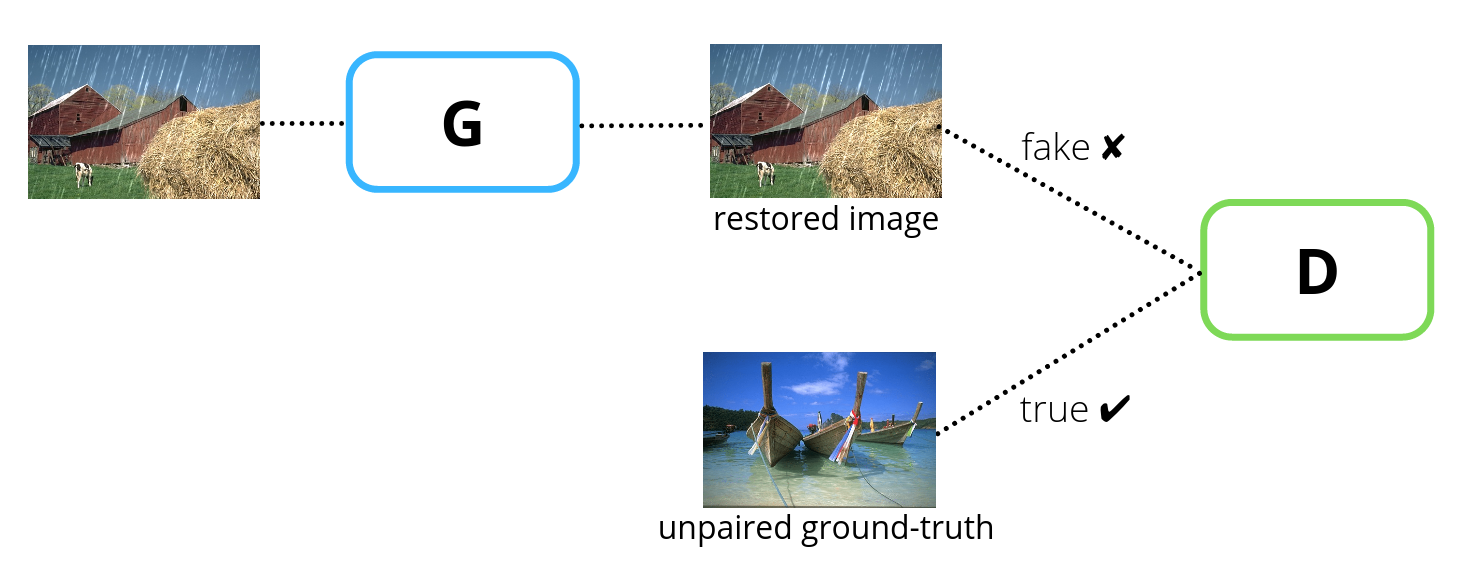
\includegraphics[scale=0.25]{./figures/unsup_GAN.png}
    \caption{Unsupervised approach for image restoration through a GAN framework.}
    \label{fig: unsup_GAN}
\end{figure}
\newpage
\section{Goal}
As part of our proposal, we are motivated to develop a ViT-GAN image restoration model for unpaired corrupted datasets (unsupervised learning).
\section{Challenges}
\subsection*{Self supervision with GAN}
\par Training restoration generator $G$ with adversarial cost alone may introduce visual artifacts in certain regions of the generated restored output, but the clean image discriminator $D$ can still end up classifying it as real data rather than generated data, which harmfs the restoration performance.
\par In our experiment we could successfully train a self supervised GAN model to restore noisy unpaired noisy-clean MNIST images. This task becomes much more difficult when using color natural images. Although, the noise is being removed from the generated images, generative artifacts are introduced in the output of the generator. Moreover, the colors between the input and the generated output are inconsistent. Suggesting that a style transfer has occurred between the unpaired training sets.
\subsection*{ViT GANs}
ViT are relatively new in the computer vision field. The challenge is that GAN training becomes highly unstable when coupled with ViTs, and that adversarial training is frequently hindered by high-variance gradients (or spiking gradients) \cite{bai2021transformers} in the later stage of discriminator training. Furthermore, conventional regularization methods such as gradient penalty, spectral normalization cannot resolve the instability issue even though they are proved to be effective for CNN-based GAN models. As unstable training is uncommon in the CNN-based GANs training with appropriate regularization, this presents a unique challenge to the design of ViT-based GANs.
